\documentclass[
hf
]{ceurart}
%\usepackage[scale=MatchLowercase]{cascadia-code}
%\DeclareFontSeriesDefault[tt]{md}{sl}
%\DeclareFontSeriesDefault[tt]{bf}{r}
%\usepackage[zerostyle=d,scaled=.94]{newtxtt}
%\usepackage{notocondensed-mono}
\usepackage{svg}
\usepackage[scaled=.8,nomap]{FiraMono}
\usepackage{minted}
%\usepackage{cprotect}
\usemintedstyle{friendly}
\usepackage{listings}
\usepackage{hyperref}
%\usepackage{microtype}
\lstset{basicstyle=\ttfamily}
\lstdefinestyle{default}{
  float=tp,
  floatplacement=tbp
}
\lstdefinelanguage{SPARQL}
{
  morekeywords={PREFIX,CONSTRUCT,SELECT,GRAPH,OPTIONAL,UNION,FROM,DISTINCT,WHERE,FILTER,GROUP,ORDER,%
  LIMIT,BY,IN,AS,SERVICE,BIND,count,geof:aggUnion,geof:collect,geof:lineMerge,geof:lineMerge,.,;,\,},
  alsoletter={:,.,;,\,},
  %otherkeywords={?,*,+},
  emph={url:text,spatial:intersectBoxGeom,spatial:withinBoxGeom,json:unnest,xml:unnest,%
  spatial:nearbyGeom,xml:parse},
  %emphstyle={\bfseries\itshape},
  emphstyle={\bfseries\slshape},
  emph={[2]strdt,json:path,iri,concat,geof:lineMerge,spatialF:transformSRS,geof:buffer,%
  spatialF:transformSRS,geof:sfIntersects,geof:simplifyDp,if,str,spatialF:transformDatatype,json:js,%
  coalesce,replace,sys:getenv,xml:path},
  emphstyle={[2]\itshape},
  sensitive=true, % keywords are not case-sensitive
  morecomment=[l]{\#}, % l is for line comment
  moredelim=[s][]{<}{>},
  %morecomment=[s][]{<}{>},
  morestring=[b]", % defines that strings are enclosed in double quotes
  %morestring=[b]', % defines that strings are enclosed in single quotes
  showstringspaces=false,
}
\newcommand\verbsparql[1]{\lstinline[keepspaces=true,language=SPARQL]{#1}}
% \makeatletter
% % improved URL link typesetting
% \def\UrlBreaks{\do\.\do\\\do\/\do\!\do\_\do\|\do\;\do\>\do\]%no @
%  \do\)\do\,\do\?\do\'\do+\do\=\do\#}%
% \def\UrlBigBreaks{\do\/\do@url@hyp}%add /
% \def\UrlSpecials{\do\/{\Url@slash}\do\ {\Url@space}\do\%{\Url@percent}\do\^^M{\Url@space}%
%    \Url@force@Tilde}%
% \def\Url@slash{\@ifnextchar/{\mathchar47\kern-.11em}%
%    {\mathchar47\penalty\UrlBigBreakPenalty}}
% \makeatother

\usepackage{caption}
\newenvironment{mintedlisting}{\captionsetup{type=lstlisting}}{}
\captionsetup[lstlisting]{singlelinecheck=false,font={small,sf},labelfont=bf}
\usepackage{cleveref}

\usepackage[base,ngerman,british]{babel}
\hyphenation{RDF-isation RDF-ised Geo-YASGUI}

\usepackage{relsize}
\newcommand{\CoyPu}{\textsc{\textsl{{\larger C\kern-1pt}oyPu}}\xspace}

\usepackage[]{todonotes}\setuptodonotes{inline}
\usepackage{fnpct}
\usepackage{awesomebox}
\usepackage{footnote}
\makesavenoteenv{tabular}
\newcommand{\infobox}[1]{%
  \awesomebox{0pt}{\raisebox{3mm}{\small\faInfo}}{gray}{{\small #1}}}
\newcommand{\infoboxcont}[1]{%
  \awesomebox{0pt}{\raisebox{3mm}{\small\!}}{gray}{{\small #1}}}
\newcommand{\lurl}[1]{\guilsinglleft\url{#1}\guilsinglright}
\usepackage{alphalph}
% \deffootnote{1.3ex}{0pt}{%
% \textsuperscript{\thefootnotemark}%
% }
\usepackage[export]{adjustbox}
\newcounter{prodtable}
\renewcommand{\theprodtable}{\alph{prodtable}}
\newcommand{\gmark}[1]{\refstepcounter{prodtable}\label{gtab:#1}\hyperlink{gtab:#1}{\textsuperscript{\theprodtable}}}
\newcommand{\gtarget}[1]{\hypertarget{gtab:#1}{\ref{gtab:#1}}}
\newcommand{\new}{\textsuperscript{+}}
\newcommand{\old}{\makebox[\widthof{\new}]{}}
% \usepackage{lastpage}
% \renewcommand{\lastpage}{\pageref{LastPage}}


\begin{document}

\title{Base Platform for Knowledge Graphs with Free Software}

\copyrightyear{2023}
\copyrightclause{Copyright for this paper by its authors.
  Use permitted under Creative Commons License Attribution 4.0
  International (CC BY 4.0).}
\conference{D2R2'23: International Workshop on Data-driven Resilience Research,
  May 28, 2023, Hersonissos}
%\fnmark[1]
\author[]{Simon Bin}[%
email=sbin@informatik.uni-leipzig.de%
]
\author[]{Claus Stadler}[]
%\author[]{Lorenz Bühmann}[]
%\author[2]{Nils Steinert}[email=nils.steinert@implisense.com]
\author[]{Norman Radtke}[]
%\author[3]{Jan Reineke}[email=jan.reineke@hitec-hamburg.de]
\author[]{Kurt Junghanns}[]
% \author[]{Kirill Bulert}[]
\author[]{Sabine Gründer-Fahrer}[]
\author[]{Michael Martin}[]
\address[]{Institute of Applied Informatics (InfAI), Leipzig}
%\address[2]{Implisense GmbH, Berlin}
%\address[3]{Hamburger Informatik Technologie-Center e.V. (HITeC), Hamburg}
%\nonumnote{note}

%% Footnotes
%\cortext[1]{Corresponding author.}
%\fntext[1]{These authors contributed equally.}

\begin{abstract}
We present an Open Source base platform for the \CoyPu knowledge graph project in the resilience domain. We report on our experiences with several tools which are used to create, maintain, serve, view and explore a modular large-scale knowledge graph, as well as 
the adaptions that were necessary to enable frictionless interaction from both performance and usability perspectives.
For this purpose, several adjustments had to be made. We provide a broad view of different programs which are of relevance to this domain. We demonstrate that while it is already possible to achieve good results with free software, there are still several pain points that need to be addressed. Resolution of these issues is often not only a matter of configuration but requires modification of the source code as well.
\end{abstract}

\begin{keywords}
Free software \sep Architecture \sep Platform \sep RDF Knowledge Graphs \sep Crisis Informatics
\end{keywords}

\maketitle

\setlength{\aweboxleftmargin}{0.06\linewidth}\setlength{\aweboxcontentwidth}{0.9\linewidth}
%\renewcommand{\thefootnote}{\textit{\alphalph{\value{footnote}}}}

\section{Introduction} % @Sabine

Semantic knowledge graphs (KGs) nowadays not only have become a key asset for search engines but are at the centre of numerous applications, for instance, in data analytics, question answering, recommendation systems, and decision support. 

Current interest from research communities as well as industries and administration rests on the capability of KGs to capture comprehensive machine-readable knowledge in application scenarios and their strengths in integrating, managing and exploiting information from heterogeneous data sources at scale. One especially interesting application scenario for KGs is crisis and resilience research. Semantic KGs can play a crucial role in increasing transparency of, for instance, economic value chains and in understanding the complex mechanisms of crisis factors at a global level. 

Although methodologies and strategies for building knowledge graphs vary based on the specific conditions and requirements of individual use cases, the creation, utilisation, and maintenance of KGs involve several common necessities and corresponding implementation phases. These processes have been discussed for more than twenty years~\cite{Gruninger1995-MethodologyFT, Noy2001-Ontology101, SurezFigueroa2012-TheNeonMethodology, Auer2012-lod-life-cycle}. While general approaches for KG development and maintenance are proposed, limited guidance regarding the selection of efficient tools for implementing these methodologies is available.

\deffootnote{1.3ex}{0pt}{%
\textsuperscript{\thefootnotemark}%
}

Knowledge graph engineering must address additional challenges in today's rapidly evolving landscape. Firstly, contemporary knowledge graphs should adhere to Linked Open Data requirements, such as the FAIR~\cite{wilkinson2016fair} data principles (Findable, Accessible, Interoperable, and Reusable) and the 5-star Open Data Model\footnote{\url{https://5stardata.info/}}. These standards ensure that the resulting knowledge graphs can be easily discovered, understood, and integrated with other datasets, promoting data sharing and collaboration across various domains. Secondly, knowledge graph engineering projects often involve teams with diverse backgrounds and expertise levels in ontology authoring. Consequently, the tools used for KG engineering must cater to both ontology experts and domain-specific specialists, facilitating effective \emph{real-time} collaboration and allowing all team members to contribute meaningfully to the development and maintenance of the knowledge graph.

We aim to create a knowledge graph-based platform for managing and exploring supply chain data. The platform will offer customised views for scientists, engineers, and decision-makers to foster collaboration and interaction with the knowledge graph. Our goal is to enable users to analyse complex data, make informed decisions, and contribute to a resilient economy.


% note: ceurart has a caption macro that does not respect textwidth/minipage env, so we need to manually
% \newline minipage figure labels

\section{Related work}

Recent studies~\cite{Hur2021, hitzler_review_2021, zhu_multi-modal_2022, ryen_building_2022, tamasauskaite_defining_2023} have shown that there are many different approaches for building specific KGs. Limitations are often faced regarding the approaches' scalability, metadata and ontology management, entity resolution and fusion, incremental updates, and quality assurance~\cite{Hofer2023}. 

While certain commercial tools like metaphactory\gmark{metaphactory} or the Enterprise Knowledge Graph Platform\gmark{eccenca} claim to offer comprehensive, all-in-one solutions, free and open-source alternatives often only address specific aspects. Consequently, users seeking to employ free and open-source tools must combine multiple applications and platforms to arrive at a complete knowledge graph platform. 

When embarking on the creation of a custom stack for knowledge graph and ontology engineering, a valuable starting point for discovering relevant tools are link collections. Two notable lists in this domain include the Awesome Knowledge Graph\footnote{\url{https://github.com/totogo/awesome-knowledge-graph}} and the Awesome Semantic Web\footnote{\url{https://github.com/semantalytics/awesome-semantic-web}} repositories on GitHub. However, it is crucial to be aware that despite being curated, these lists may still suffer from link rot, leading to outdated or non-functional resources.
%
The previously popular list hosted on the W3C website\footnote{\url{https://www.w3.org/2001/sw/wiki/Category:RDF_or_OWL_Browser}} is rather outdated, with only 4 out of 21 listed tools still operable at the time of writing in the category of ``RDF or OWL browser''  (LodView\gmark{lodview}, Rhizomer~\cite{garcia2022rhizomer}, Structured Data Linter, and VocBench~\cite{stellato2020vocbench}).
%
Refer to \autoref{tab:overview} for an overview of the tools mentioned in this paper.

\begin{figure}
%\begin{minipage}[t]{.54\textwidth}
    \centering
    %https://docs.google.com/drawings/d/1P6-gHaQKUB7YyJZsQCRotTvux4DlrOYS7dOkUiAyJ-A/edit?usp=sharing
    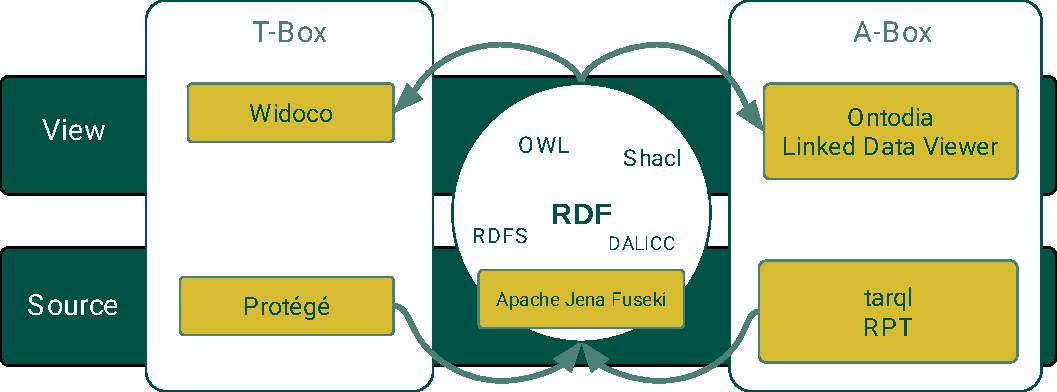
\includegraphics[width=.9\textwidth]{overview_coy_rdf.pdf}
    \caption{Overview of our solution architecture}
    \label{fig:architecture}
%\end{minipage}\hfill%
\end{figure}

\section{Solution and other tools}

In the following, we will show how we tackle the previous concerns with free and open-source tools. Our solution and the utilised tools are shown in \autoref{fig:architecture}.

\paragraph{Ontology authoring.}\label{para:onto}
Part of creating knowledge graphs involves creating a schema (ontology) for your data. We used the venerable Protégé~\cite{musen2015protege} for this purpose. We looked but failed to find other comparable OWL\footnote{Web Ontology Language, \url{https://www.w3.org/TR/owl2-overview/}} authoring tools. While working on the ontology together with the partners, we found the best working approach to discuss one step of ontology evolution in a group and then designate one person to implement the change. Afterwards, the change could be reviewed on a source code control system. For the latter, it should also be ensured that all engineers are using the same version of Protégé, this will ensure that the textual difference of changes to the ontology is minimal and limited to the actual changes implemented.

\infobox{The commercial tool TopBraid Composer\gmark{topbraid} might provide an alternative, but we did not evaluate it (the free edition would crash when trying to open our ontology). VocBench might also be a candidate (we did not try it.)}

To document and visualise our ontologies, we used the Widoco~\cite{garijo2017widoco} documentation tool in an automated fashion from the command line.  Widoco extends LODE and also includes WebVOWL~\cite{lohmann2015webvowl}, a graph-based visualisation of the ontology document. You can inspect the result on \lurl{https://schema.coypu.org/}. We have created a \emph{pipeline} that updates our documentation whenever the ontology files are changed in the Git source code repository on GitLab\footnote{Source code for the pipeline script on \href{https://gitlab.com/coypu-project/coy-ontology/}{gitlab.com/coypu-project/coy-ontology} in the supplements folder}.

\infobox{Potential alternatives for Widoco include pyLODE\gmark{pylode} or JOD\gmark{jod}. In our initial attempt, JOD did not readily handle multiple ontologies and there was no way to reference the entities in the documentation. It was also hiding too much information behind tabs, obstructing the view at a glance. PyLODE did not support our annotations out of the box. These issues might be fixable by spending some time on the templates, however.}

% note: ceurart has a caption macro that does not respect textwidth/minipage env, so we need to manually
% \newline minipage figure labels
\begin{figure}
%\begin{minipage}[t]{.44\textwidth}
    \centering
    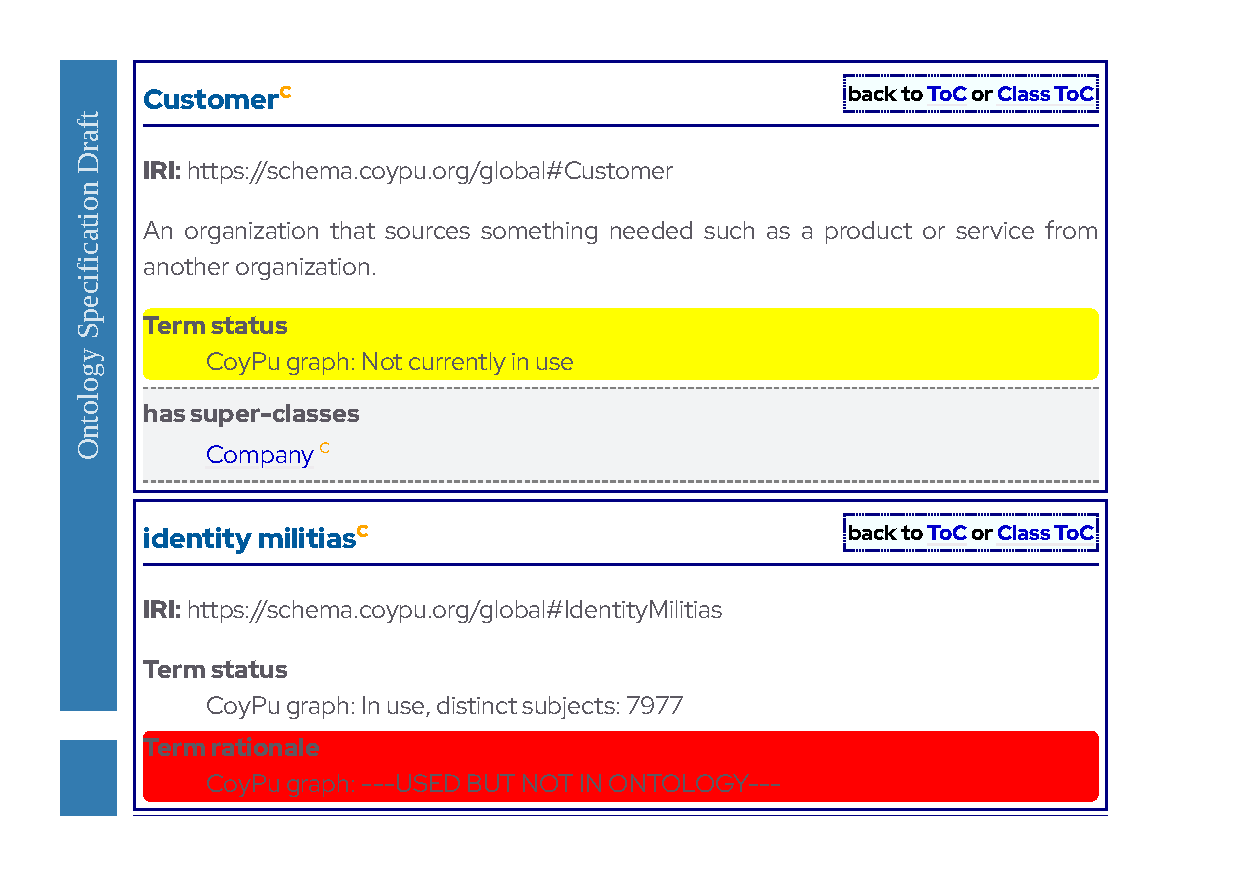
\includegraphics[width=\textwidth,trim={1cm 1cm 1cm 3.5cm},clip]{CoyPu Ontology.pdf}
    \caption{CoyPu Ontology documentation %\newline
    enriched with usage information, hinting at %\newline
    incomplete ontology}
    \label{fig:ontology_doc}
%\end{minipage}%
\end{figure}

The availability of the ontology documentation helps in locating the classes and properties to use when creating the mappings (see \nameref{para:mapping}).
To further enhance the usefulness of our documentation for the modelling workflow, we enrich the ontology documentation with usage statistics from the actual instance data (see \autoref{fig:ontology_doc}). In the example, the term ``identity militias'' has been found in use in our knowledge graph, but not yet described in the ontology, whereas the term ``Customer'' is contained in the ontology but not (yet) used in the knowledge graph. Calculation of the usage statistics is done using the RDF Processing Toolkit (RPT)\gmark{rpt} with a set of VoID~\cite{alexander2011describing}-generating SPARQL queries\footnote{\url{https://gitlab.com/coypu-project/dataset-stats/-/tree/main/compact}}.

\infobox{Automated pipelines that run automatically whenever changes to your ontology are committed to a source code control system, require integration with the source code control system. There are two common ways to realise pipelines. One is to use the platform-specific CI/CD pipelines\footnote{Forgejo/Woodpecker: \url{https://woodpecker-ci.org/docs/usage/intro},\newline GitLab: \url{https://docs.gitlab.com/ee/ci/quick_start/},\newline GitHub: \url{https://github.blog/2022-02-02-build-ci-cd-pipeline-github-actions-four-steps/}}, the other is using a Webhook event\footnote{\url{https://progrium.github.io/blog/2007/05/03/web-hooks-to-revolutionize-the-web/}} to trigger the start of an external pipeline.}

To further increase the quality of our ontology, we have started to implement RDFUnit~\cite{rdfunit} rules that check the ontology details and version. Another standard with growing adoption is the Shapes Constraint Language (SHACL)\footnote{\url{https://www.w3.org/TR/shacl/}}, which might be validated for example using pySHACL~\cite{pyshacl} or Jena SHACL\gmark{jenashacl}.

%rdfunit bei sparql-basierten tests vorteile, pyshacl strikt shacl-spezifikation

\paragraph{Mapping structured data to RDF data.}\label{para:mapping}
A big part of our knowledge graph is not our original creation, but rather the mapping and integration, combination, and refinement of existing data sources. Most of the data sources we used are structured data, for example in XML, GML, JSON, CSV formats or data returned by Web APIs. Other parts of the data were also extracted and semantified from unstructured or semi-structured data like news articles.

Several different tools were used by the different project partners, for example Tarql\gmark{tarql}, RPT or Morph-KGC~\cite{arenas2022morph}. Each tool was chosen by the familiarity of the expert user and applicability to the data source that is to be mapped. Tarql for instance is an excellent choice to map CSV to RDF. RPT on the other hand can easily process CSV, JSON, and XML input files as well as web APIs and remote services using SPARQL, and Morph-KGC can map CSV or connect to SQL databases using RML.

\infobox{There is a plenitude of mapping tools that can be found. Other projects that might be worth investigating are SPARQL-Generate~\cite{lefrancois_eswc_2017}, RML~\cite{dimou2014rml}, SPARQL Anything~\cite{daga2021facade}.}

We found the concise syntax of SPARQL as used in Tarql and RPT to be very refreshing compared to the rather detailed way in which R2RML mapping documents are written. Especially the way to register custom functions in RML is quite heavy-handed, whereas RPT allows defining such functions using either JavaScript or Java annotations\footnote{\url{https://docs.oracle.com/javase/6/docs/technotes/guides/language/annotations.html}}. We also tested some commercial web-form based mapping editor, but found it to be rather cumbersome when having to edit and refine the mappings compared to a good old programmers' text editor. 

Further tools used by our partners include Named entity recognition from text using Falcon~2.0~\cite{falcon20} as well as many custom-written programs\footnote{\url{https://docs.coypu.org/ExternalRepositories.html}}. For some of these, the Python RDFLib\gmark{rdflib} was a popular choice when producing RDF data.

\paragraph{Dereference and visualise the Graph.}\label{para:visual}
In our experience in the \CoyPu project, we found it extremely helpful to grasp the Semantic Web concepts when the IRIs are dereferenceable, i.e. you can open the IRIs of your graph entities in the browser. Users and experts alike want to see and understand what is ``in'' the graph. The \emph{classes and properties} are dereferenceable through the use of Widoco and publishing the ontology documentation at the same location as the Ontology IRI. To make the \emph{data} dereferenceable and browseable, tools like Trifid\gmark{trifid} and LodView can be used. It was easy to start Trifid with the Docker image provided by the authors. However, the default view is a bit bland. There is a great overview of tools presented in~\cite{regalia2017phuzzy}, but we found that at the time of writing only LodView and Trifid were still available.

\begin{figure}
%\begin{minipage}[t]{.47\textwidth}
    \centering
    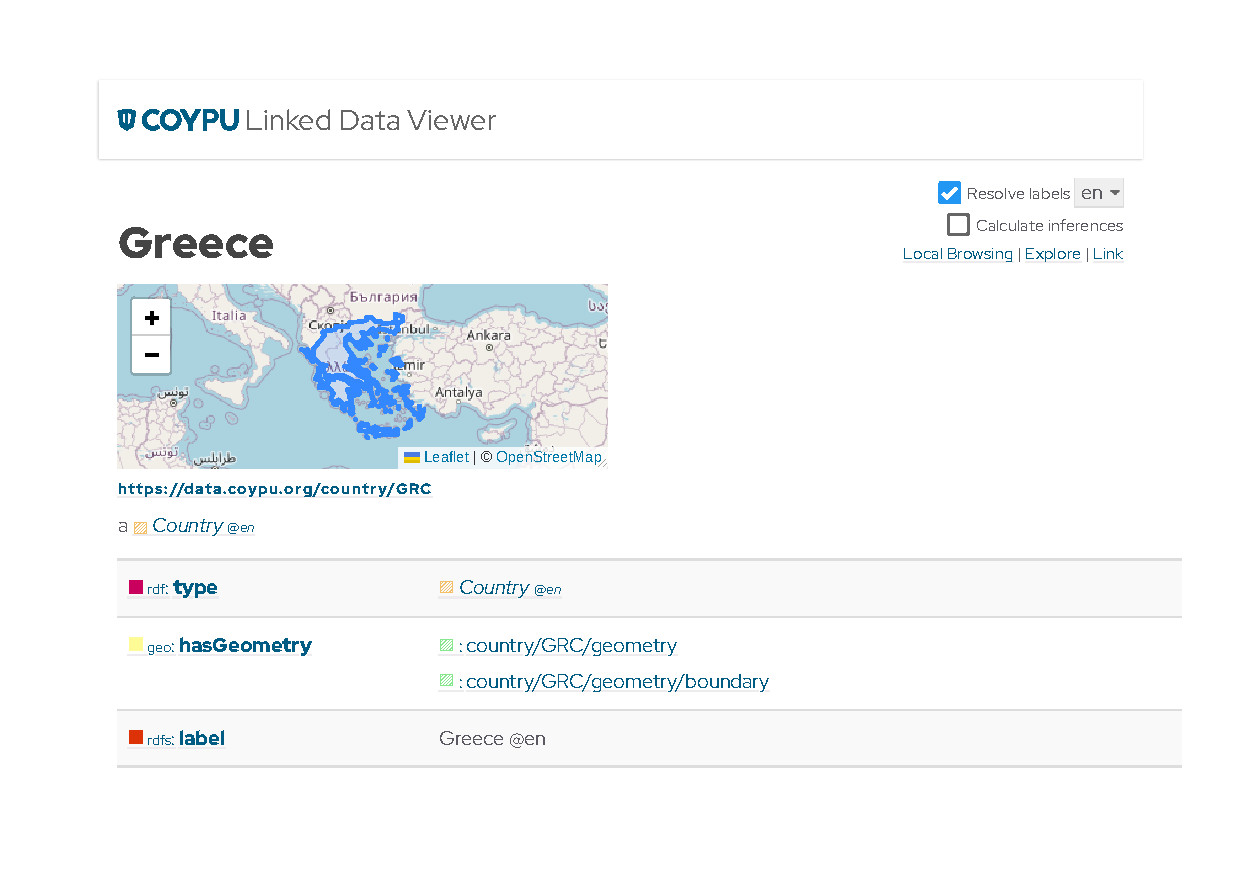
\includegraphics[width=\textwidth,trim={1.8cm 2cm 1.8cm 1cm},clip]{Linked Data Viewer.pdf}
    \caption{Linked data viewer showing some %\newline
    subject triples}
    \label{fig:ldv}
%\end{minipage}\hfill%
\end{figure}

Our solution for IRI dereferencing (see \autoref{fig:ldv}) is built on top of the Trifid rendering component\gmark{ldv}. Compared to Trifid, we have extended the code for full client-side querying, a map widget for resources with geospatial data, rendering of inverse relations (similar to LodView), source attribution (useful to know which data set the entity is from), lazy pagination for many property values, label resolution and language switching, colour cards for name-spaces and optional inferencing. Furthermore, we support browser-based authentication for password-protected graph databases. 

\begin{figure}
%\begin{minipage}[t]{.52\textwidth}
    \centering
    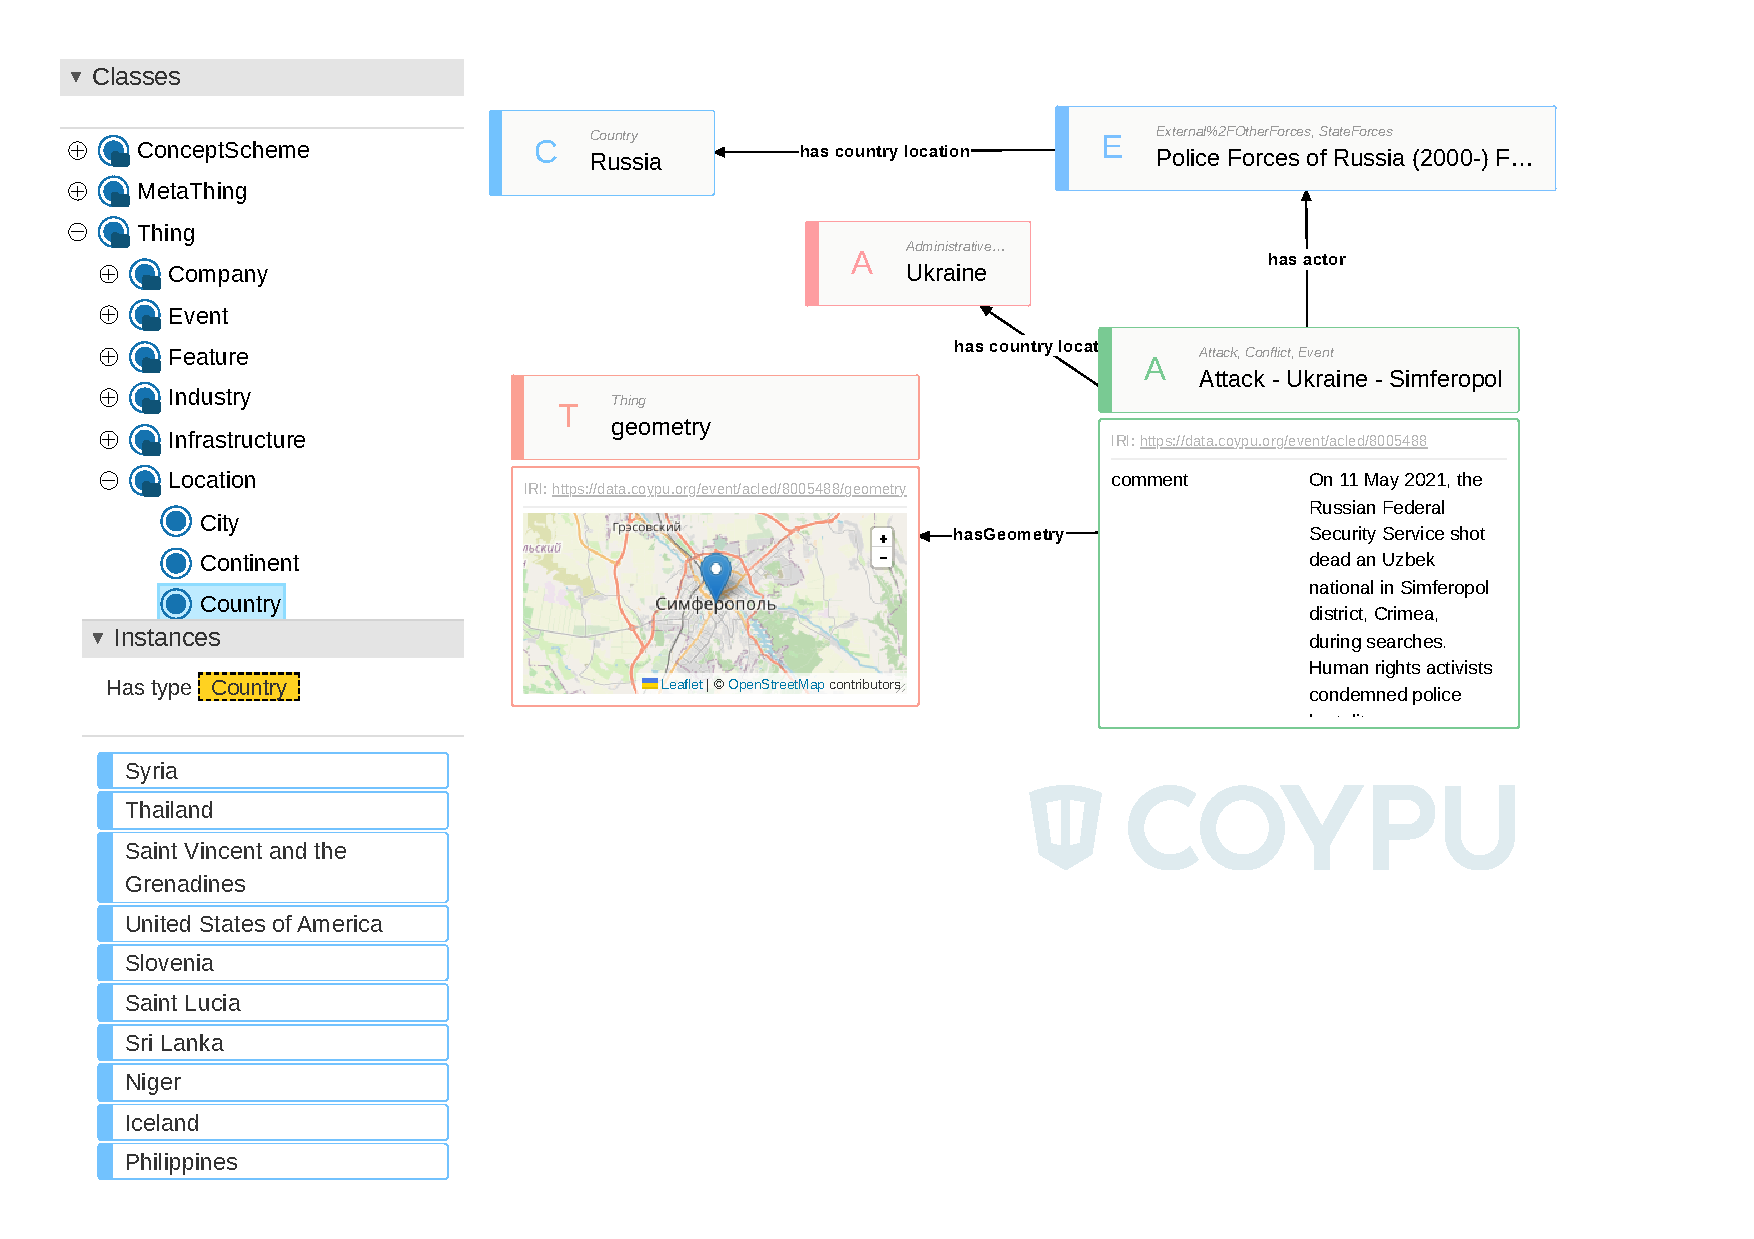
\includegraphics[width=\textwidth,trim={1cm 4cm 2cm 1cm},clip]{Graph Explorer.pdf}
    \caption{Ontodia Graph Explorer with Map widget}
    \label{fig:graph_explorer}
%\end{minipage}%
\end{figure}

To make the graph explorable and the graph-based nature understandable, we have found the Ontodia Graph Explorer (see \autoref{fig:graph_explorer}) \cite{mouromtsev2015simple}. It allows one to interactively add existing entities from the knowledge graph to a drawing area on the screen, and will automatically add the links between entities. It can also show the Ontology schema in a tree fashion and will show a list of instances of the selected ontology class. We refined the graph explorer with a geo-spatial map widget and the possibility to hide obstructive properties. Further, we included meta-data schema and concept schema in the class tree. As a convenience, we have also integrated a link into the Linked Data Viewer which will add the current entity to the graph explorer, and we have made it possible to share created knowledge graph diagrams with other users through custom links. 

\infobox{LODmilla~\cite{micsik2014lodmilla} would be another knowledge graph browser, but it does not receive much attention these days. Another tool for exploring knowledge graphs is the RDF surveyor~\cite{vega2019linked}. It extends the Trifid/LodView concept with more exploratory options. (We did not evaluate these tools.)}

For interactive testing of SPARQL queries and their results, we found YASGUI~\cite{rietveld2017yasgui} and GeoYASGUI~\cite{beek2017geoyasgui} very convenient. Thanks to the integration of Google Charts and Openstreetmap\footnote{\url{https://www.openstreetmap.org}, implemented with Leaflet:~\url{https://leafletjs.com/}} map widget, it is possible to present and verify the SPARQL results of geospatial data and numeric data easily.

\paragraph{Documentation and Dataset catalogue.}\label{para:docs}

To provide project documentation, we make use of Just the Docs\gmark{justthedocs}. The documentation can be written in Markdown in our source control system and is then deployed on \lurl{https://docs.coypu.org/} using a pipeline. The configuration has been extended with a ``Try it!'' link on SPARQL queries\footnote{\url{https://gitlab.com/coypu-project/skynet/platform-exhibits/-/tree/main/just-the-docs}}, so that these can be tried out directly on the Jena Fuseki User Interface.

Additionally, a tabular listing of our data catalogue content is published at \lurl{https://datasets.coypu.org/} by automatically executing SPARQL queries on our knowledge graph and rendering the result to Markdown. This is done by feeding the SPARQL CSV output~\cite{seaborne2013csv} into \texttt{csvlook}\gmark{csvlook}.

The data catalogue itself is hand-created in RDF/Turtle format and collects all the details about the externally sourced data that is being used in the \CoyPu project. This includes licensing information, links to the data source, the target RDF graph where this data set is loaded and a link to the Data Licenses Clearance Center~\cite{pellegrini2018automated}\footnote{\url{https://www.dalicc.net/}} (DALICC) licence where available. We plan to record further meta-data into our catalogue, such as the tools involved in transforming the original data into RDF data.

\infobox{The DALICC offers a RESTful web service that supports \emph{automated clearance of rights} thus supporting the \emph{legally secure and time-efficient re-utilisation of third-party data sources}.
The service is also named DALICC and the source code can be found on GitHub.
It is possible to run your own instance of DALICC but some features like the usage of a remote SPARQL endpoint are missing at the moment.
We also consider extending the service with a feature that helps to examine the rights and permission of data, derived from multiple datasets (e.g. via SPARQL queries).}

\paragraph{Hosting and serving the knowledge graph.}\label{para:server}
We use Apache Jena~\cite{carroll2004jena} Fuseki backed by Apache Jena TDB2, both combined making a full-fledged SPARQL Endpoint for scripts and programs to work with. Getting started is mostly straightforward, for a simple deployment you can download the Apache Jena Fuseki release and start it (Java is required). 

Extensive customisation has been added to our Jena Fuseki. First of all, we configured geo-spatial\footnote{\url{https://jena.apache.org/documentation/geosparql/geosparql-assembler}} and Lucene~\cite{bialecki2012apache} text index in Fuseki\footnote{\url{https://jena.apache.org/documentation/query/text-query.html\#text-dataset-assembler}}. The endpoint for the Graph Store Protocol\footnote{\url{https://www.w3.org/TR/sparql11-http-rdf-update/}} was moved from the Fuseki-default to a \texttt{/data} sub-path, to stop inadvertent dumps of the full graph. The endpoint has been access-restricted using Apache Shiro that is included in Fuseki\footnote{\url{https://jena.apache.org/documentation/fuseki2/fuseki-security.html}} (we hope to make it publicly available at a later date).

We identified a performance bottleneck involving SPARQL \texttt{FROM} queries and implemented a \texttt{FROM}-as-\texttt{GRAPH} filter for Jena. Concerning the geospatial data, we added GeoSPARQL functions such as \texttt{lat}, \texttt{lon} (to access the latitude and longitude of a point), \texttt{centroid} and \texttt{aggUnion} (from the upcoming GeoSPARQL 1.1 standard~\cite{car2022geosparql}) and \texttt{simplifyDp} (to simplify a geometry) or \texttt{lineMerge}\footnote{\url{https://github.com/opengeospatial/ogc-geosparql/issues/402}} functions, which we have suggested to the Open Geospatial Consortium for consideration. Additionally, the geospatial index was reprogrammed to work on a per-graph level rather than on the whole data set, and we also implemented a Fuseki service to recompute the geo-index of individual graphs at run-time\gmark{fmod-geospatial}. The initial loading time of the index was also heavily improved due to a custom serialisation format.
%
To aid in RDFS\footnote{\url{http://www.w3.org/TR/rdf-schema/}} reasoning and \texttt{owl:sameAs}~\cite{motik2015handling} resolution, we have implemented two new SPARQL-\texttt{SERVICE} based RDFS and sameAs inferencers. They are also conveniently exposed in our linked data viewer (see \nameref{para:visual}).
%
These additional functions are implemented in our JenaX\gmark{jenax} extension modules for Apache Jena.


\paragraph{Server Infrastructure.}\label{para:infra}
The knowledge graph and the associated processes cannot conveniently operate on free resources. To deploy our knowledge graph, we have a physical server with  250~GiB main memory, of which the Apache Jena Fuseki server is using 50~GiB. According to one of the Jena maintainers\footnote{\url{https://lists.apache.org/thread/43vo5pdgfy0mst2pl6ppyyf65bwf7yb2}}, per TDB2 database approx. 2~GiB heap should be assigned (we have configured 10~databases). We have configured the Java heap space to 32~GiB\footnote{\texttt{java -Xmx} command line flag} (after having experimented with smaller values, but those were found insufficient when executing larger \texttt{CONSTRUCT} or \texttt{UPDATE} queries).

The on-disk database files take currently 200~GiB of disk space, which amounts to 700~million ($7\cdot 10^8$) triples spread across 39~graphs. For the spatial index for GeoSPARQL, 300~MiB of disk space is used for our 4~million ($4\cdot 10^6$) geometries. The database files are stored on 4~SATA QLC SSDs operating in a software RAID. Fuseki is accessing the database files using memory-mapped I/O. Scanning through the whole index takes 200~seconds and scanning the whole literal table takes 50~minutes.

To create the initial database, we used RPT to convert all the output from our various mapping tools into N-Quads format and then the \texttt{xloader} script included in Fuseki. We did this after testing all the various loaders provided by Fuseki and determining that this script works best for our hardware/configuration. Altogether, it takes 8~hours for our system to convert the source RDF files into a Fuseki TDB2 database. The break-down is as follows: 3h~20m for mapping the data, 4h~20m for loading into TDB2, 1~minute to calculate the statistics for the query optimiser, 7~minutes to calculate the geospatial index for GeoSPARQL queries, 20~minutes to calculate a Lucene index for full-text search on the RDFS labels and just short of 1~minute to reload the database. (All times, sizes, and triple counts are approximate.)
%
\footnote{An initial stumbling block for us was that the server was originally provided to the project with a ZFS RAID-1 filesystem~\cite{bonwick2003zettabyte} on Ubuntu. Despite database-specific tuning\footnotemark{} we were unable to make it work satisfactorily. The system Input-output load became unbearably high so we had to reinstall the system using the ext4\footnotemark{} filesystem.}
\addtocounter{footnote}{-2}%
\stepcounter{footnote}\footnotetext{\url{https://openzfs.github.io/openzfs-docs/Performance\%20and\%20Tuning/Workload\%20Tuning.html}} 
\stepcounter{footnote}\footnotetext{\url{https://www.kernel.org/doc/Documentation/filesystems/ext4.txt}}


\section{Conclusion}

Many free and open-source software components have been created by the community when it comes to knowledge graph serving and preparation. Nevertheless, it can be challenging to set up the individual software components and configure them in the right way to work together. We had to manually configure nearly all of the components, which requires a diverse skill set ranging from Docker, YAML, JSON, and Bash, to SPARQL, JavaScript, and Java. 

The remaining pain points are the long loading times and the query performance for more complex SPARQL queries as well as missed automatic optimisations when using the full-text search. Other issues could be improved, such as the per-graph Geo-index, but could be further enhanced for example by implementing a self-updating geo-index.

We gave impulses to heavily optimise the speed of certain specific queries such as the named graph list\footnote{\url{https://github.com/apache/jena/pull/1655}} and raised other issues as we met them. Other improvements have been contributed directly by us, such as speed-ups for certain path query patterns, geospatial queries, or a whole new bulk SPARQL service and cache implementation. Yet other improvements such as the per-graph geo-index are still work-in-progress in our fork of Apache Jena, or part of our JenaX extension modules for Apache Jena. We plan to upstream our changes if possible, and to provide a docker compose file for easy reproducing of the set-up described in this paper.

\begin{acknowledgments}
The authors acknowledge the financial support by the Federal Ministry for Economic Affairs and Energy of Germany in the project Coypu (project number 01MK21007[A-L]).
\end{acknowledgments}

{%\small
\bibliography{main} %
}
\clearpage

\begin{table}[p]\vskip-.5\baselineskip
    \centering
    \caption{\vskip-\baselineskip \hspace{\widthof{\textbf{Table 1:}}}Overview of the tools mentioned in this work; \new repository updated after May 2022}
    \begin{tabular}{clccl}
    \toprule
        Ref. & Name & Category & Licence & Repository / Website \\
        \midrule 
        \multicolumn{4}{c}{\textbf{Commercial}} & \\
         \gtarget{metaphactory} & metaphactory & &  & \href{https://metaphacts.com/product}{metaphacts.com} \\
         \gtarget{eccenca} & \multicolumn{2}{l}{\makecell[l]{Enterprise Knowledge \\ Graph Platform}} &  & \href{https://eccenca.com/products/enterprise-knowledge-graph-platform-corporate-memory}{eccenca.com} \\
         \gtarget{topbraid} & TopBraid Composer & Authoring &  & \href{https://franz.com/agraph/tbc/}{franz.com/agraph/tbc} \\
         \multicolumn{4}{c}{\textbf{Free software}} & \\
         \cite{stellato2020vocbench}\new & VocBench & Authoring & BSD-3-Clause & \href{https://vocbench.uniroma2.it/}{vocbench.uniroma2.it} \\
         \cite{musen2015protege}\new & \makecell[l]{Protégé \\ \footnotesize Version 5.6.1} & Authoring & BSD-2-Clause & \href{https://protege.stanford.edu/}{protege.stanford.edu} \\
         \cite{garijo2017widoco}\new & \makecell[l]{Widoco \\ \footnotesize Version 1.4.17} & Docu. & Apache-2.0 & \href{https://github.com/dgarijo/Widoco}{github.com/dgarijo/Widoco} \\
         \gtarget{pylode}\new & pyLODE & Docu. & \makecell{GPL-3.0 / \\ BSD-3-Clause} & \href{https://github.com/rdflib/pyLODE}{github.com/rdflib/pyLODE} \\
         \gtarget{jod}\new & JOD & Docu. & MIT & \href{https://github.com/eccenca/jod}{github.com/eccenca/jod} \\ 
         \gtarget{justthedocs}\new & Just the Docs & Docu. & MIT & \href{https://github.com/just-the-docs/just-the-docs\#just-the-docs}{github.com/just-the-docs/just-the-docs} \\
         \gtarget{csvlook}\new & csvkit / csvlook & Docu. & MIT & \href{https://csvkit.readthedocs.io/en/latest/scripts/csvlook.html}{csvkit.readthedocs.io} \\
         \gtarget{rpt}\new & \makecell[l]{RDF Processing \\ Toolkit} & Mapping+ & Apache-2.0 & \makecell[l]{\href{https://github.com/SmartDataAnalytics/RdfProcessingToolkit}{github.com/SmartDataAnalytics/} \\ \href{https://github.com/SmartDataAnalytics/RdfProcessingToolkit}{RdfProcessingToolkit}} \\
         \gtarget{tarql}\old & Tarql & Mapping & BSD-2-Clause  & \href{https://tarql.github.io/}{tarql.github.io} \\
         \cite{arenas2022morph}\new & Morph-KGC & Mapping & Apache-2.0 & \href{https://morph-kgc.readthedocs.io}{morph-kgc.readthedocs.io} \\
         \cite{lefrancois_eswc_2017}\new & SPARQL-Generate & Mapping & Apache-2.0 & \href{https://ci.mines-stetienne.fr/sparql-generate/}{ci.mines-stetienne.fr/sparql-generate} \\
         \cite{dimou2014rml}\new & RML & Mapping & MIT & \href{https://rml.io/}{rml.io} \\
         \cite{daga2021facade}\new &  SPARQL Anything & Mapping & Apache-2.0 & \href{https://sparql-anything.cc/}{sparql-anything.cc} \\
         \cite{falcon20}\old & \makecell[l]{Falcon \\ \footnotesize Version 2.0} & NER & MIT & \href{https://labs.tib.eu/falcon/falcon2/}{labs.tib.eu/falcon/falcon2} \\
         \cite{rdfunit}\new & RDFUnit & Quality & Apache-2.0 & \href{https://github.com/AKSW/RDFUnit}{github.com/AKSW/RDFUnit} \\
         \cite{pyshacl}\new & pySHACL & Quality & Apache-2.0 & \href{https://github.com/RDFLib/pySHACL}{github.com/RDFLib/pySHACL} \\
         \gtarget{jenashacl}\new & Jena SHACL & Quality & Apache-2.0 & \href{https://jena.apache.org/documentation/shacl/}{jena.apache.org/documentation/shacl/} \\
         \gtarget{lodview}\new & LodView & Deref. & MIT & \href{https://github.com/LodLive/LodView}{github.com/LodLive/LodView} \\
         \gtarget{trifid}\new & Trifid & Deref. & Apache-2.0 & \href{https://github.com/zazuko/trifid}{github.com/zazuko/trifid} \\
         \gtarget{ldv}\new & \makecell[l]{Linked Data \\ Viewer} & Deref. & MIT & \makecell[l]{\href{https://github.com/AKSW/Linked-Data-Viewer}{github.com/AKSW/} \\ \href{https://github.com/AKSW/Linked-Data-Viewer}{Linked-Data-Viewer}} \\
         \cite{garcia2022rhizomer}\new & Rhizomer & Explore & GPL-3.0 & \href{https://rhizomik.net/about}{rhizomik.net} \\
         \multirow{2}{*}{\cite{mouromtsev2015simple}\old} & \multirow{2}{*}{\makecell[l]{Ontodia \\ Graph Explorer}} & \multirow{2}{*}{Explore} & LGPL-2.1+ & \href{https://github.com/zazuko/graph-explorer}{github.com/zazuko/graph-explorer} \\
         \multicolumn{4}{r@{}}{\footnotesize changes on} & \footnotesize \url{https://github.com/AKSW/graph-explorer} \\
         \cite{micsik2014lodmilla}\old & LODmilla & Explore & Apache-2.0 & \makecell[l]{\href{https://lodmilla.sztaki.hu/lodmilla/?id=hhaeuotogto2k565i7644folcg}{lodmilla.sztaki.hu} \\ \href{https://github.com/dsd-sztaki-hu}{github.com/dsd-sztaki-hu}} \\
         \cite{vega2019linked}\old & RDF surveyor & Explore & Apache-2.0 & \makecell[l]{\href{http://tools.sirius-labs.no/rdfsurveyor/}{tools.sirius-labs.no/rdfsurveyor} \\ \href{https://github.com/guiveg/rdfsurveyor}{github.com/guiveg/rdfsurveyor}} \\
         \cite{rietveld2017yasgui}\new & YASGUI & Explore & MIT & \href{https://yasgui.triply.cc/}{yasgui.triply.cc} \\
         \cite{beek2017geoyasgui}\old & GeoYASGUI & Explore & MIT & \makecell[l]{\href{https://github.com/Triply-Dev/YASGUI.YASR-deprecated/tree/geo}{github.com/Triply-Dev/} \\ \href{https://github.com/Triply-Dev/YASGUI.YASR-deprecated/tree/geo}{YASGUI.YASR-deprecated/tree/geo}} \\
         \gtarget{rdflib}\new & \makecell[l]{RDFLib \\ \footnotesize Version 6.2.0} & & BSD-3-Clause &  \href{https://rdflib.readthedocs.org/}{rdflib.readthedocs.org} \\
         \multirow{2}{*}{\cite{carroll2004jena}\new} & \multirow{2}{*}{\makecell[l]{Apache Jena \\ \footnotesize  Version 4.8.0}} & & Apache-2.0  & \href{https://jena.apache.org/}{jena.apache.org} \\
         \multicolumn{4}{r@{}}{\footnotesize work-in-progress on} & \footnotesize \url{https://github.com/AKSW/jena} \\
         \gtarget{fmod-geospatial}\new & \makecell[l]{ Geo-Service \\ \footnotesize for Jena Fuseki } & & Apache-2.0 & \href{https://github.com/AKSW/fuseki-mods}{github.com/AKSW/fuseki-mods} \\
         \gtarget{jenax}\new & JenaX & & Apache-2.0 & \href{https://github.com/Scaseco/jenax}{github.com/Scaseco/jenax} \\
         \bottomrule
         \end{tabular}
    \label{tab:overview}
\end{table}

\end{document}
